
\section{Recommender algorithm}
Recommender systems and especially those utilizing on content-based methods are derived from information retrieval (IR).\citep[p.~92-99]{lops:2011}
Also Rocchio's algorithm for relevance feedback origins from information retrieval.\citep[p.~178]{manning:2009}
In order to implement Rocchio's algorithm there is a brief introduction of the information retrieval basics and its methodology related to Rocchio's algorithm.

\subsection{Information retrieval}
\index{information retrieval}
\citeauthor{manning:2009} describe Information Retrieval in their book as process of ``finding material [\dots] of an unstructured nature [\dots] that satisfies an information need from within a large collection."\citep[p.~1]{manning:2009}\\
In general IR and RS are very similar and many technologies and findings of IR can be transfered to RS.
Since IR systems are build to handle unstructured data and transform them into a form that is easier to handle for computer systems one can adopt the method to RS input data such as items.\citep[p.~21-23]{ricci:2011}
There are various ways IR systems interpret data.
However this thesis will focus on one common method (and the theory it is based on) called ``tf-idf-vectors" which is a prerequisite for Rocchio's algorithm.\citep[p.~93]{lops:2011}

IR systems are built to handle ``unstructured data".
Unstructured data is information bundled within a document (document is the IR related term for what is understood as item by RS) without any clear semantical structure.\citep[p.~1-3]{manning:2009}
%The data within a document
IR systems can extract all relevant terms from a document.
A term may resemble an attribute of an item such as its colour or brand.
%The way of retrieving terms from a unstructured document is out of scope for this thesis but there is a brief example in figure~\ref{fig:TermRetrieving}.\\
For this section the IR vocabulary will be adopted.
This means, that items will be called documents and attributes will be known as terms.

\iffalse
% this figure might not be accurate :/
% therefore it will not appear in the final thesis
\begin{figure}[h]
    \center
    %\lstset{style=customHTML}
    \begin{lstlisting}
<html>
    <head><title>Online shop</title></head>
    <body>
        <img src="/img/p_42.jpg" alt="FancyBrand's product"/>
        <table>
            <tr><td>Colour</td><td>green</td></tr>
            <tr><td>Price</td><td>24,95 &euro;</td></tr>
            <tr><td>Brand</td><td>FancyBrand</td></tr>
        </table>
    </body>
</html>
    \end{lstlisting}
    \rowcolors{1}{\dustRowFirst}{\dustRowSecond}
    \begin{tabular}{ l }
        \rowcolor{\dustRowHead}
        \textbf{Terms}\\\hline
        green\\
        24,95 \&euro;\\
        FancyBrand%\\\hline
    \end{tabular}
    \caption{Retrieving Terms from a HTML document.}
    \label{fig:TermRetrieving}
\end{figure}
\fi


\subsection{Weighting}
\label{sec:weighting}
As already mentioned a document can be be described as a collection of terms.
The process of locating terms within a document is currently taken for granted.
When a user queries for a specific term one has to find all relevant document including this term.
In addition an order regarding the document's significance will be required.
The significance of a term within a document is defined by its weight.\citep[p.~117]{manning:2009}

While primitive IR methods such as boolean retrieval only check for the mere existence of a queried term within a document, weighting can give more precise results regarding the terms significance in a document.\citep[p.~109]{manning:2009}

\paragraph{Term frequency}
\label{sec:tf}
\index{Term Frequency}
A simple method to quantify a term's importance within a document is the so called term frequency.
This concept is based on the assumption that the frequency of a term $t$ indicates its importance within a document $d$.
It is denoted as $\text{tf}_{t,d}$ where $t$ resembles the term an $d$ the document.
The number of occurrences of $t$ within $d$ can be directly interpreted its term frequency.\citep[p.~117]{manning:2009}

For products of an online shop and its resulting term frequency may look like as described in figure~\ref{fig:tfweighting}.

\begin{figure}[h]

    \begin{quote}
        Document $\text{d}1$ with identified terms underlined:\\
        \underline{blouse} \underline{blue} \underline{55} Euro. \underline{55} cm by size \underline{S}. 100\% \underline{Polyester}
    \end{quote}

    \center
    \vspace{5mm}
    \rowcolors{0}{\dustRowFirst}{\dustRowSecond}
    \begin{tabular}{ l l }
        \rowcolor{\dustRowHead}
        \multicolumn{2}{c}{Term frequency}\\\hline
        $\text{tf}_{\text{blouse},\text{d1}}$       & 1\\
        $\text{tf}_{\text{blue},\text{d1}}$         & 1\\
        $\text{tf}_{\text{55},\text{d1}}$           & 2\\
        $\text{tf}_{\text{S},\text{d1}}$            & 1\\
        $\text{tf}_{\text{Polyester},\text{d1}}$    & 1\\
    \end{tabular}

    \caption{Term frequency weighting}
    \label{fig:tfweighting}
\end{figure}

\paragraph{Inverse document frequency}
\label{sec:idf}
\index{Inverse Document Frequency}
In some domains special terms will often appear multiple times within a document and therefore have high term frequency weight without giving any explanatory value.\citep[p.~117]{manning:2009}
Documents resembling clothing offered by an online shop may always include the name of the store as term.
Since the user already explicitly searches at this store, the relevance of this term is rather low.
In order to transfer this to weighting, inverse document weighting (idf) has been introduced.
Idf will scale down the weighting of terms which appear in every document.
To do so, an intermediate step is necessary. Before calculating the idf for a term one has to determine both the terms document frequency ($\text{df}_t$) and the total count of documents (as $N$).
The number of documents in which a term appears can be directly interpreted as the term's document frequency.
\citep[p.~116-118]{manning:2009}
Idf can be calculated with following formula:
\\
\begin{equation}
    \text{idf}_{t} = \log\frac{N}{\text{df}_{t}}
    \label{eq:idf-forumula}
\end{equation}
The logarithms basis isn't of great importance.\citep[p.~118]{manning:2009}
The examples in this thesis however use 10 as base.
A more explanatory example is presented by figure~\ref{fig:idfweighting}.
The example states that rare items posses a higher idf, whereas more frequent terms are rated lower.\citep[p.~118]{manning:2009}

\begin{figure}[h]
    \begin{quote}
        Total count of documents  $N$ is 500\\
        Term1 "FancyShop" appears in 500 documents\\
        Term2 "blouse" appears in 130 documents\\
    \end{quote}

    \center
    \begin{tabular}{ l | l }
        $\text{df}_{\text{FancyShop}} = 500$                                                                    & $\text{df}_{\text{blouse}} = 130$\\
        $\text{idf}_{\text{FancyShop}} = \log\frac{N}{\text{df}_{\text{FancyShop}}} = \log\frac{500}{500} = 0$  & $\text{idf}_{\text{blouse}} = \log\frac{N}{\text{df}_{\text{blouse}}} = \log\frac{500}{130} \approx 0.59$
    \end{tabular}

    \caption{Inverse document frequency weighting}
    \label{fig:idfweighting}
\end{figure}

\paragraph{Tf-Idf}
\label{sec:tfidf}
\index{TfIdf}
Both the term frequency, as well as the inverse document frequency have some drawbacks.
While term frequency may weight terms with little informative value high because they appear often (word such as ``is", ``the"), inverse document frequency can totally ignore terms by weighting them extremely low.
But it's possible to combine both \textit{tf} and \textit{idf} in order to get better weightings.
The result is called \textit{tf-idf}.\citep[p.~118-119]{manning:2009}
\begin{equation}
    \text{tf-idf}_{\text{t,d}} = \text{tf}_\text{t,d} \times \text{idf}_\text{d}
    \label{eq:tf-idf-forumula}
\end{equation}

\noindent
Figure~\ref{fig:tfidfweighting} illustrates the generation of an tf-idf weighting.
\begin{figure}[h]

    \begin{quote}
        Total number of documents $N$ is 3\\
    \end{quote}

    \center
    \rowcolors{1}{\dustRowFirst}{\dustRowSecond}
    \begin{tabular}{ l l | l l l l }
        \rowcolor{\dustRowHead}
        Term                    & Document          & tf    & df & idf   & tf-idf\\\hline
        blouse                  & $\text{doc}_1$    & 15    &  2 & 0.18  & 2.7\\
        blouse                  & $\text{doc}_2$    & 5     &  2 & 0.18  & 0.9\\
        blouse                  & $\text{doc}_3$    & 0     &  2 & 0.18  & 0\\
    \end{tabular}
    \caption{tf-idf weighting}
    \label{fig:tfidfweighting}
\end{figure}

\noindent
\citeauthor{manning:2009} describes tf-idf weighting as follows:\\
``$\text{[Tf-idf}_{\text{t,d}}\text{]}$ assigns to term $t$ a weight in document $d$ that is
\begin{enumerate}
    \item highest when $t$ occurs many times within a small number of documents
    (thus lending high discriminating power to those documents);
    \item lower when the term occurs fewer times in a document, or occurs in many
    documents (thus offering a less pronounced relevance signal);
    \item lowest when the term occurs in virtually all documents."
\end{enumerate}
\citep[p.~119]{manning:2009}

\subsection{Vector space model}
\label{sec:vectorspacemodel}
\index{VectorSpaceModel}
Any document can now be described as a vector.
Each term in a document will be directly interpreted as component of a vector.
If a term is non existent in a document, the vector component will be set to numeric zero.\citep[p.~120]{manning:2009}

Therefore IR provides methods to describe documents as vectors.
Forging a bridge back to RS the vectors can help to provide a computer representation of real world products.

The vectors of all products can be displayed in one common vector space, whereas the number of dimensions is determined by the number of vector components.
This process is known as vector space model.\citep[p.~120]{manning:2009}
An example of a two dimensional vector space model is given in figure~\ref{fig:vectorspacemodel}.


In this way any document or item can be displayed as a bunch of values.
In case of tf-idf this would be floating point values.
When trying to represent a document in computer memory (as required by \textbf{Q3}) it would be practical to simply create an array holding the values by which it is represented.
However there are many ways to implement this.
For this thesis documents have been displayed in a relative verbose way with quite a lot of meta information.
A document gets resembled by lists containing a term-name and the corresponding value.
A more detailed view is given in section~\ref{sec:content-analyzer}.

\begin{figure}[h]

    \begin{quote}
        There are three documents with following terms:\\
        Document $\text{d}_1$: $1\times \text{FancyBrand}, 2\times \text{green}$\\
        Document $\text{d}_2$: $1\times \text{FancyBrand}$\\
        Document $\text{d}_3$: $1\times \text{green}$\\
        Whereas "FancyBrand" and "green" are the document terms.


        \iffalse
        \rowcolors{1}{\dustRowFirst}{\dustRowSecond}
        \begin{tabular}{ l l | l l l l }
            \rowcolor{\dustRowHead}
            Term                    & Document          & tf    & df & idf   & tf-idf\\\hline
            FancyBrand              & $\text{doc}_1$    & 1     &  2 & 0.18  & 0.18\\
            green                   & $\text{doc}_1$    & 2     &  2 & 0.18  & 0.35\\\hline
%
            FancyBrand              & $\text{doc}_2$    & 1     &  2 & 0.18  & 0.18\\
            green                   & $\text{doc}_2$    & 0     &  2 & 0.18  & 0\\\hline
%
            FancyBrand              & $\text{doc}_3$    & 0     &  2 & 0.18  & 0\\
            green                   & $\text{doc}_3$    & 1     &  2 & 0.18  & 0.18\\
        \end{tabular}
        \fi

        \noindent
        The generic tf-idf vector representation of one of the documents above will be:\\
        $\vec{\text{v}}_{\text{generic}} = (\text{tf-idf}_{\text{FancyBrand},\text{d}_\text{generic}}, \text{tf-idf}_{\text{green},\text{d}_\text{generic}})^T$

        \noindent
        The corresponding tf-idf-vectors of the are:\\
        $\vec{\text{v}}_1 = (\text{tf-idf}_{\text{FancyBrand},\text{d}_1}, \text{tf-idf}_{\text{green},\text{d}_1})^T = (0.18, 0.35)^T$\\
        $\vec{\text{v}}_2 = (\text{tf-idf}_{\text{FancyBrand},\text{d}_2}, \text{tf-idf}_{\text{green},\text{d}_2})^T = (0.18, 0)^T$\\
        $\vec{\text{v}}_3 = (\text{tf-idf}_{\text{FancyBrand},\text{d}_3}, \text{tf-idf}_{\text{green},\text{d}_3})^T = (0, 0.18)^T$\\
    \end{quote}

    \begin{quote}
        With vector $\vec{\text{v}}_n$ as position vector describing points relative to the origin.
    \end{quote}
    \center
    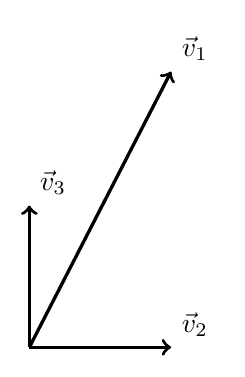
\begin{tikzpicture}
        \tkzInit[xmax=0.5,ymax=0.5,xstep=0.1,ystep=0.1]
        %\tkzAxeX[label=FancyBrand,above left=10pt]
        \tkzAxeX[label=FancyBrand, right]
        %\tkzAxeY[label=green,below right=30pt]
        \tkzAxeY[label=green,above]
        \tkzGrid
        \draw[very thick, ->] (0,0) -- (1.8,3.5) node[anchor=south west]{$\vec{\text{v}}_1$};
        \draw[very thick,latex-latex, ->] (0,0) -- (1.8,0) node[anchor=south west]{$\vec{\text{v}}_2$};
        \draw[very thick,latex-latex, ->] (0,0) -- (0, 1.8) node[anchor=south west]{$\vec{\text{v}}_3$};
    \end{tikzpicture}

    \caption{Two dimensional vector space model}
    \label{fig:vectorspacemodel}
\end{figure}


\iffalse
\subsubsection{Parametric and zone indices}
\label{sec:parametricandzoneindices}
\fi

% evtl. noch ausf\"uhren:
% - stop words (woerter die nicht gewertet werden z.b. ist, er war, ...)
% - Parametric and zones indices


\subsection{Rocchio's algorithm}
\label{sec:rocchio}
With section~\ref{sec:tfidf} and section~\ref{sec:vectorspacemodel} all requirements of Rocchio's algorithm have been described.\citep[p.~178]{manning:2009}
The next step is to specify the algorithm itself.
Rocchio's relevance feedback algorithm is classified as content-based RS.\citep[p.~92]{lops:2011}
The algorithm tries to find a vector representing a user which is similar to all item's relevant to the user.
In addition the number of non-relevant items matching the vector should be minimal.
Rocchio's algorithm originates from IR and normally utilizes a search query from a user.
This query can be used for preselecting relevant and non-relevant items.
Based on this knowledge the algorithm would refine the search query by gathering more feedback (as described in section~\ref{sec:feedback}).
% 182
\citep[p.~178-182]{manning:2009}
%One of the algorithms characteristics is the way feedback (as described in section~\ref{sec:feedback}) is treated.
Every time the user gives either positive or negative feedback, the algorithm will adapt the user vector to match the new criteria.\citep[p.~387-388]{pazzani:2007}

For implementing Rocchio's algorithm in a recommender system a user vector will be used instead of a query vector as originally intended.
\begin{equation}
    \vec{\text{q}}_m =
        \alpha \cdot \vec{\text{q}}_0
        + \beta \cdot \frac{1}{|\text{D}_\text{r}|}\sum_{\vec{\text{d}}_j\in \text{D}_\text{r}} \vec{\text{d}}_j
        - \gamma \cdot \frac{1}{|\text{D}_\text{nr}|}\sum_{\vec{\text{d}}_j\in \text{D}_\text{nr}} \vec{\text{d}}_j
\end{equation}

$\vec{\text{q}}_0$ is the old vector representing the user before he gave feedback about one of the items.
The result $\vec{\text{q}}_m$, however, is the modified vector describing the user after his most recent feedback has been taken into consideration.
For each calculation with Rocchio's algorithm $\vec{\text{q}}_0$ will always be the result $\vec{\text{q}}_m$ of the preceding calculation.
Effectively Rocchio's algorithm creates a vector that can be inserted into the vector space from section~\ref{sec:vectorspacemodel}.
With each application of Rocchio's algorithm the output vector leads to a point resembling the users preferences.
And all items close to this point can be used as possible recommendations, as they resemble attributes the user prefers.

$\text{D}_\text{r}$ is a set of all relevant item vectors, while $\text{D}_\text{nr}$ represents a set of items which are not relevant to the user.

$\alpha$, $\beta$ and $\gamma$ act as weights and can influence the importance of the old user vector, as well as of  the relevant and irrelevant documents.
The old user vector is weighted by $\alpha$.
The average of relevant documents is weighted by $\beta$ and $\gamma$ is responsible for irrelevant documents.
There are only positive values for weights allowed.
The lowest possible weight is 0.
A well established configuration for these weights is: $\alpha = 1$, $\beta = 0.75$ and $\gamma = 0.15$.
However if a RS only allows positive feedback, one can as well set $\gamma$ to 0.
\citep[p.~178-183]{manning:2009}


The weighting of $\alpha$, $\beta$ and $\gamma$ is a good way of adjusting Rocchio's algorithm as they can also be changed during run-time (whereas run-time labels the application of Rocchio's algorithm in a RS).
Even thought it is possible it remains uncertain whether adjusting Rocchio's algorithm at run-time bears any benefit or not.
This question will be further explained in section~\ref{sec:testing-findings}.
Therefore there is only a partial answer to \textbf{Q4} yet, as raison d'\^{e}tre will be discussed later.
However it adapting the algorithm at run-time is no problem at all.

\subsection{Vector space classification}
Up to this point both items and users can be represented as vector within a vector space model.
The theory of vector space classification basically states that items within a vector space model form regions with the items next to them.
These different regions do not overlap and resemble classes of document.
\citep[p.~298-291]{manning:2009}
Information retrieval as area of research provides some methods for determining vectors that are strongly connected within the vector space model.
This can be used to find items which are near a given user vector since they should have similar characteristics as the user vector.
The more similar a user vector and a item are, the more likely the item provides use for the user.
\citep[p.~298-291]{manning:2009}

One of IRs methods which can be used is k-nearest-neighbours (kNN).
It identifies $k$ nearest neighbours next to a given vector within the vector space model (whereas $k$ is the number of results one expects).
This behaviour can be used for identifying items which can be recommended to a user as queried in \textbf{Q5}.
A slightly more in-depth explanation of kNN will be given in section~\ref{sec:filtering-component} when kNN is implemented.
%
